\subsection{Task 5: permutation lattice}

Monotone translation is not at all realistic. 
However, instead of experimenting with phrase-based distortion-based permutation mechanism, you will experiment with preordered input.
We are providing you with lists containing up to 100 permutations of the sentences in \texttt{dev.en} and with phrase tables that are suitable for those permutations. 
The data available for this task is summarised in Table \ref{tab:data-preordered}.
You are not directly provided with lattices of preordered input, instead you are provided with lists such as illustrated in Figure \ref{fig:n-best}.


\begin{table}\centering
\begin{tabular}{l p{9cm} }
\textbf{File}   & \textbf{Description} \\
\texttt{dev.enpp.nbest} & Up to 100-best permutations of each sentence in \texttt{dev.en} \\
\texttt{rules.engp-ja.dev.tgz}  & A collection of phrase pairs relevant to permutations of each source sentence\\
\texttt{weights.lattice} & Parameters of a linear model for lattice translation \\
\end{tabular}
\caption{\label{tab:data-preordered}Data for lattice translation.}
\end{table}


There is a trivial way to represent a list using automata/transducers which are non-deterministic. See Figure \ref{fig:permutations}, where I have represented each permutation using an independent path to an independent final state. I have weighted the path by weighting its final arc and I am using negative log-probabilities.

\begin{figure}[h]\centering
\begin{tabular}{l l}
0.7 & \texttt{the dog black } \\
0.2 & \texttt{dog black the} \\
0.1 & \texttt{the black dog} \\
\end{tabular}
\caption{\label{fig:n-best}Example of list of permutations (and their probabilities).}
\end{figure}


The downside is that there is no packing and the representation is rather inefficient.
Consider finite-state operations that may alleviate that problem (e.g. determinisation and  minimisation). Figure \ref{fig:pi-det-min} illustrates a much more efficient representation: observe that even though the topology of the automaton changed, the paths are exactly the same and so are their negative log-probabilities.\footnote{You will note that the weights of the paths have been somehow distributed along the arcs towards the initial node. This is the result of a standard operation called \emph{push}. Pushing weights towards the initial node is usually a good idea because one can reason about the total weight of a path earlier on. This is particularly useful when decoding with A$^*$ or beam search.}

\begin{figure}[h]\centering
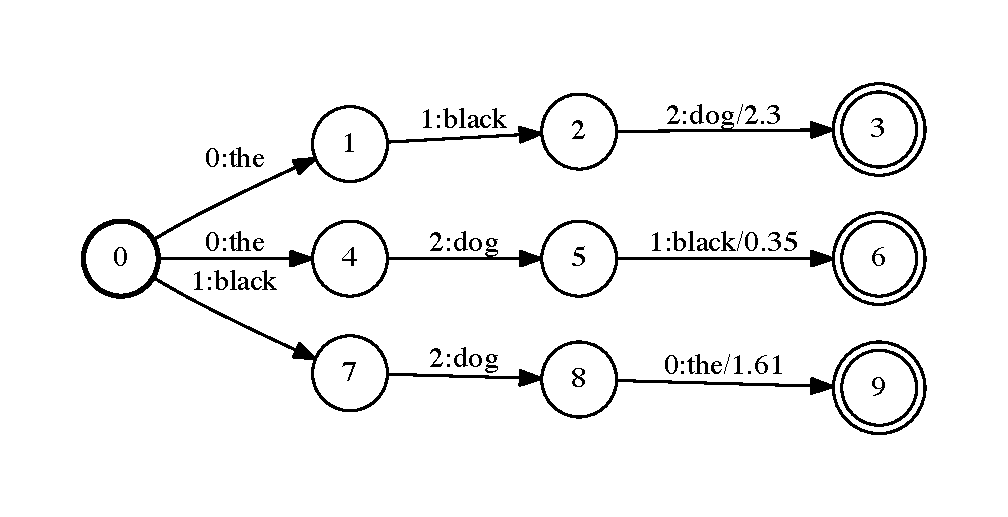
\includegraphics[scale=0.5]{permutations-list.pdf}
\caption{\label{fig:permutations}List of permutations as a non-deterministic transducer.}
\end{figure}


In order to discriminate alternative permutations, we will add a feature to our linear model. 
This feature is the negative log-probability of the permutation and the model parameter associated with it is called \texttt{LatticeCost}.
Table \ref{tab:task5} summarises the task. 

\begin{figure}[h]\centering
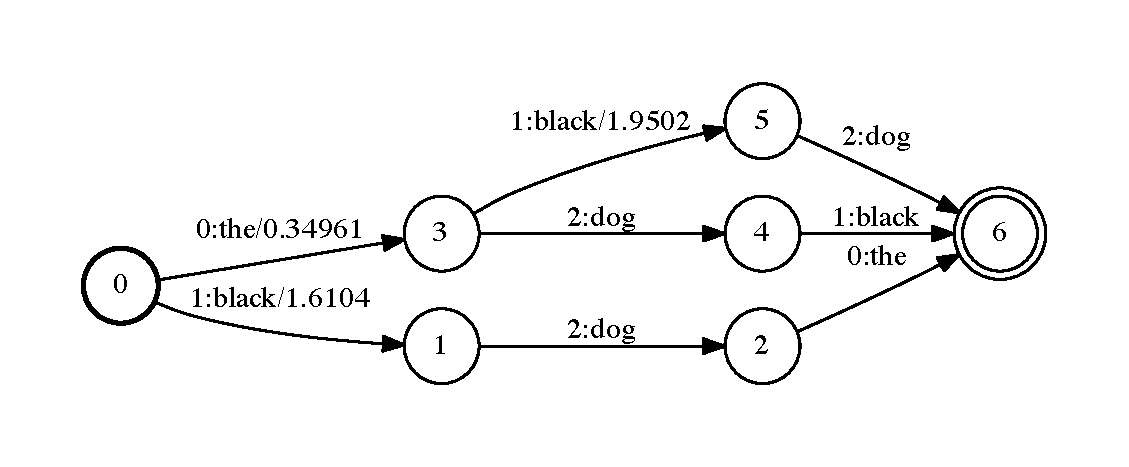
\includegraphics[scale=0.5]{permutations-lattice.pdf}
\caption{\label{fig:pi-det-min}Permutations packed in a deterministic transducer.}
\end{figure}

\begin{table}[h]\centering
\begin{tabular}{l p{12cm}}
\textsc{Task}   &  pack permutations into weighted lattices\\
\textsc{Input}  &  up to 100 permutations per source sentence \\
\textsc{Output} &  a permutation lattice per source sentence\\
\textsc{Submit} &  nothing to submit here\\  
\textsc{Report} & discuss the strategies for packing: e.g. determinisation and minimisation\\
\end{tabular}
\caption{\label{tab:task5}Task 5 summarised}
\end{table}

